\documentclass{grand-jeu}
\usepackage{wrapfig}

\titre[76]{Plateforme coopérative (Variante)}
\categorie{Solidaire}

\begin{document}

\begin{liste-materiel}
\materiel{1 balle de tennis / ping pong / balle de jonglage}
\materiel{Un anneau sur lequel peut être posé la balle}
\materiel{Autant de morceaux de ficelle (de 2M) que de joueurs}
\materiel{un promontoire (type paquet de Pringles vide rempli de cailloux) qui passe à l’intérieur de l’anneau}
\end{liste-materiel}

\begin{regles}
\begin{wrapfigure}{r}{3cm}
\vspace{-1cm}
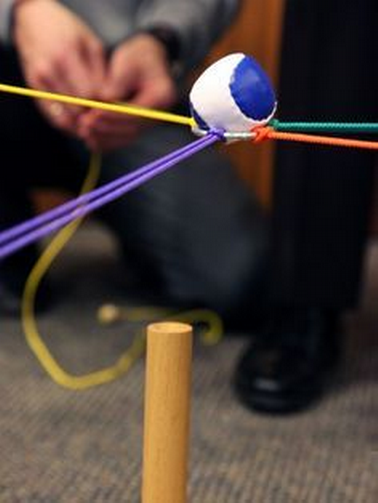
\includegraphics[height=5cm]{4-Solidaire-rouge/sources/76.png}
\end{wrapfigure}

But du jeu : placer la balle sur le promontoire.

Chaque joueur tient une ficelle (tendue) et doit poser la balle sur le promontoire sans faire tomber ni la balle ni le promontoire.

Si les joueurs réussissent à faire passer la balle jusqu'au bout dans le temps imparti, ils gagnent des b-dures.
\end{regles}


\begin{imaginaire}

\end{imaginaire}

\begin{moments-stop}
\end{moments-stop}


\end{document}